\documentclass{slide}

% Could comment out animate package for GitHub commited version to reduce slide compilation time.
% Note: The animate package seems sensitive to currency of the version of LaTeX used to compile a document.
\usepackage{animate}

% Following two packages are only needed if final slide with manually created table is used.
%\usepackage{colortbl}
%\usepackage{changepage}

\usepackage{setspace}
% From setspace use \setstretch.
% \setstretch requires \\ at end of paragraphs.

%\usepackage{pgfpages}
%\setbeameroption{show notes on second screen}

\title{Deployment Strategies}
\subtitle{CSSE6400}
\author{Richard Thomas}
\date{\week{11}}


\begin{document}

\maketitle

\begin{frame}{Branching \& Deployment Strategies}
  \vspace{1pt}
  {\huge
    \begin{itemize}
        \item Branching Strategies
        \vspace{8pt}
        \item Deployment Strategies
	    \begin{itemize}
	        \LARGE\item[$-$] Recreate Deployment
	        \LARGE\item[$-$] Rolling Deployment
	        \LARGE\item[$-$] Blue/Green Deployment
	        \LARGE\item[$-$] Canary Deployment
	        \LARGE\item[$-$] A/B Deployment
	        \LARGE\item[$-$] Shadow Deployment
	    \end{itemize}
    \end{itemize}
  }
\end{frame}
\note{There isn't any one perfect deployment strategy.}

\definition{Branching}{Copying the trunk to allow separate and parallel development.}
\note[itemize]{
    \item Branches deviate from the trunk.
    \item A few different branching strategies.
}

\begin{frame}{Branching Strategies}
  \vspace{1pt}
  {\huge{\setstretch{1.25}
    \begin{itemize}
        \item GitHub Flow
        \item GitLab Flow
        \item Release Branches
    \end{itemize}
  }}
\end{frame}
\note{Branching strategies supporting deployment strategies.}

\begin{frame}{GitHub Flow \cite{github-flow}}
    \vspace{1pt}
    \begin{columns}
    \column{0.45\textwidth}
      {\LARGE
        \vspace{-5mm}
        \begin{itemize}
            \item {\setstretch{0.95} Main is always deployable\\}
            \item Create branch
            \item Make changes
            \item Create pull request
            \item Resolve issues
            \item Merge pull request
            \item Delete branch
        \end{itemize}
      }
    \column{0.55\textwidth}
        \centering
        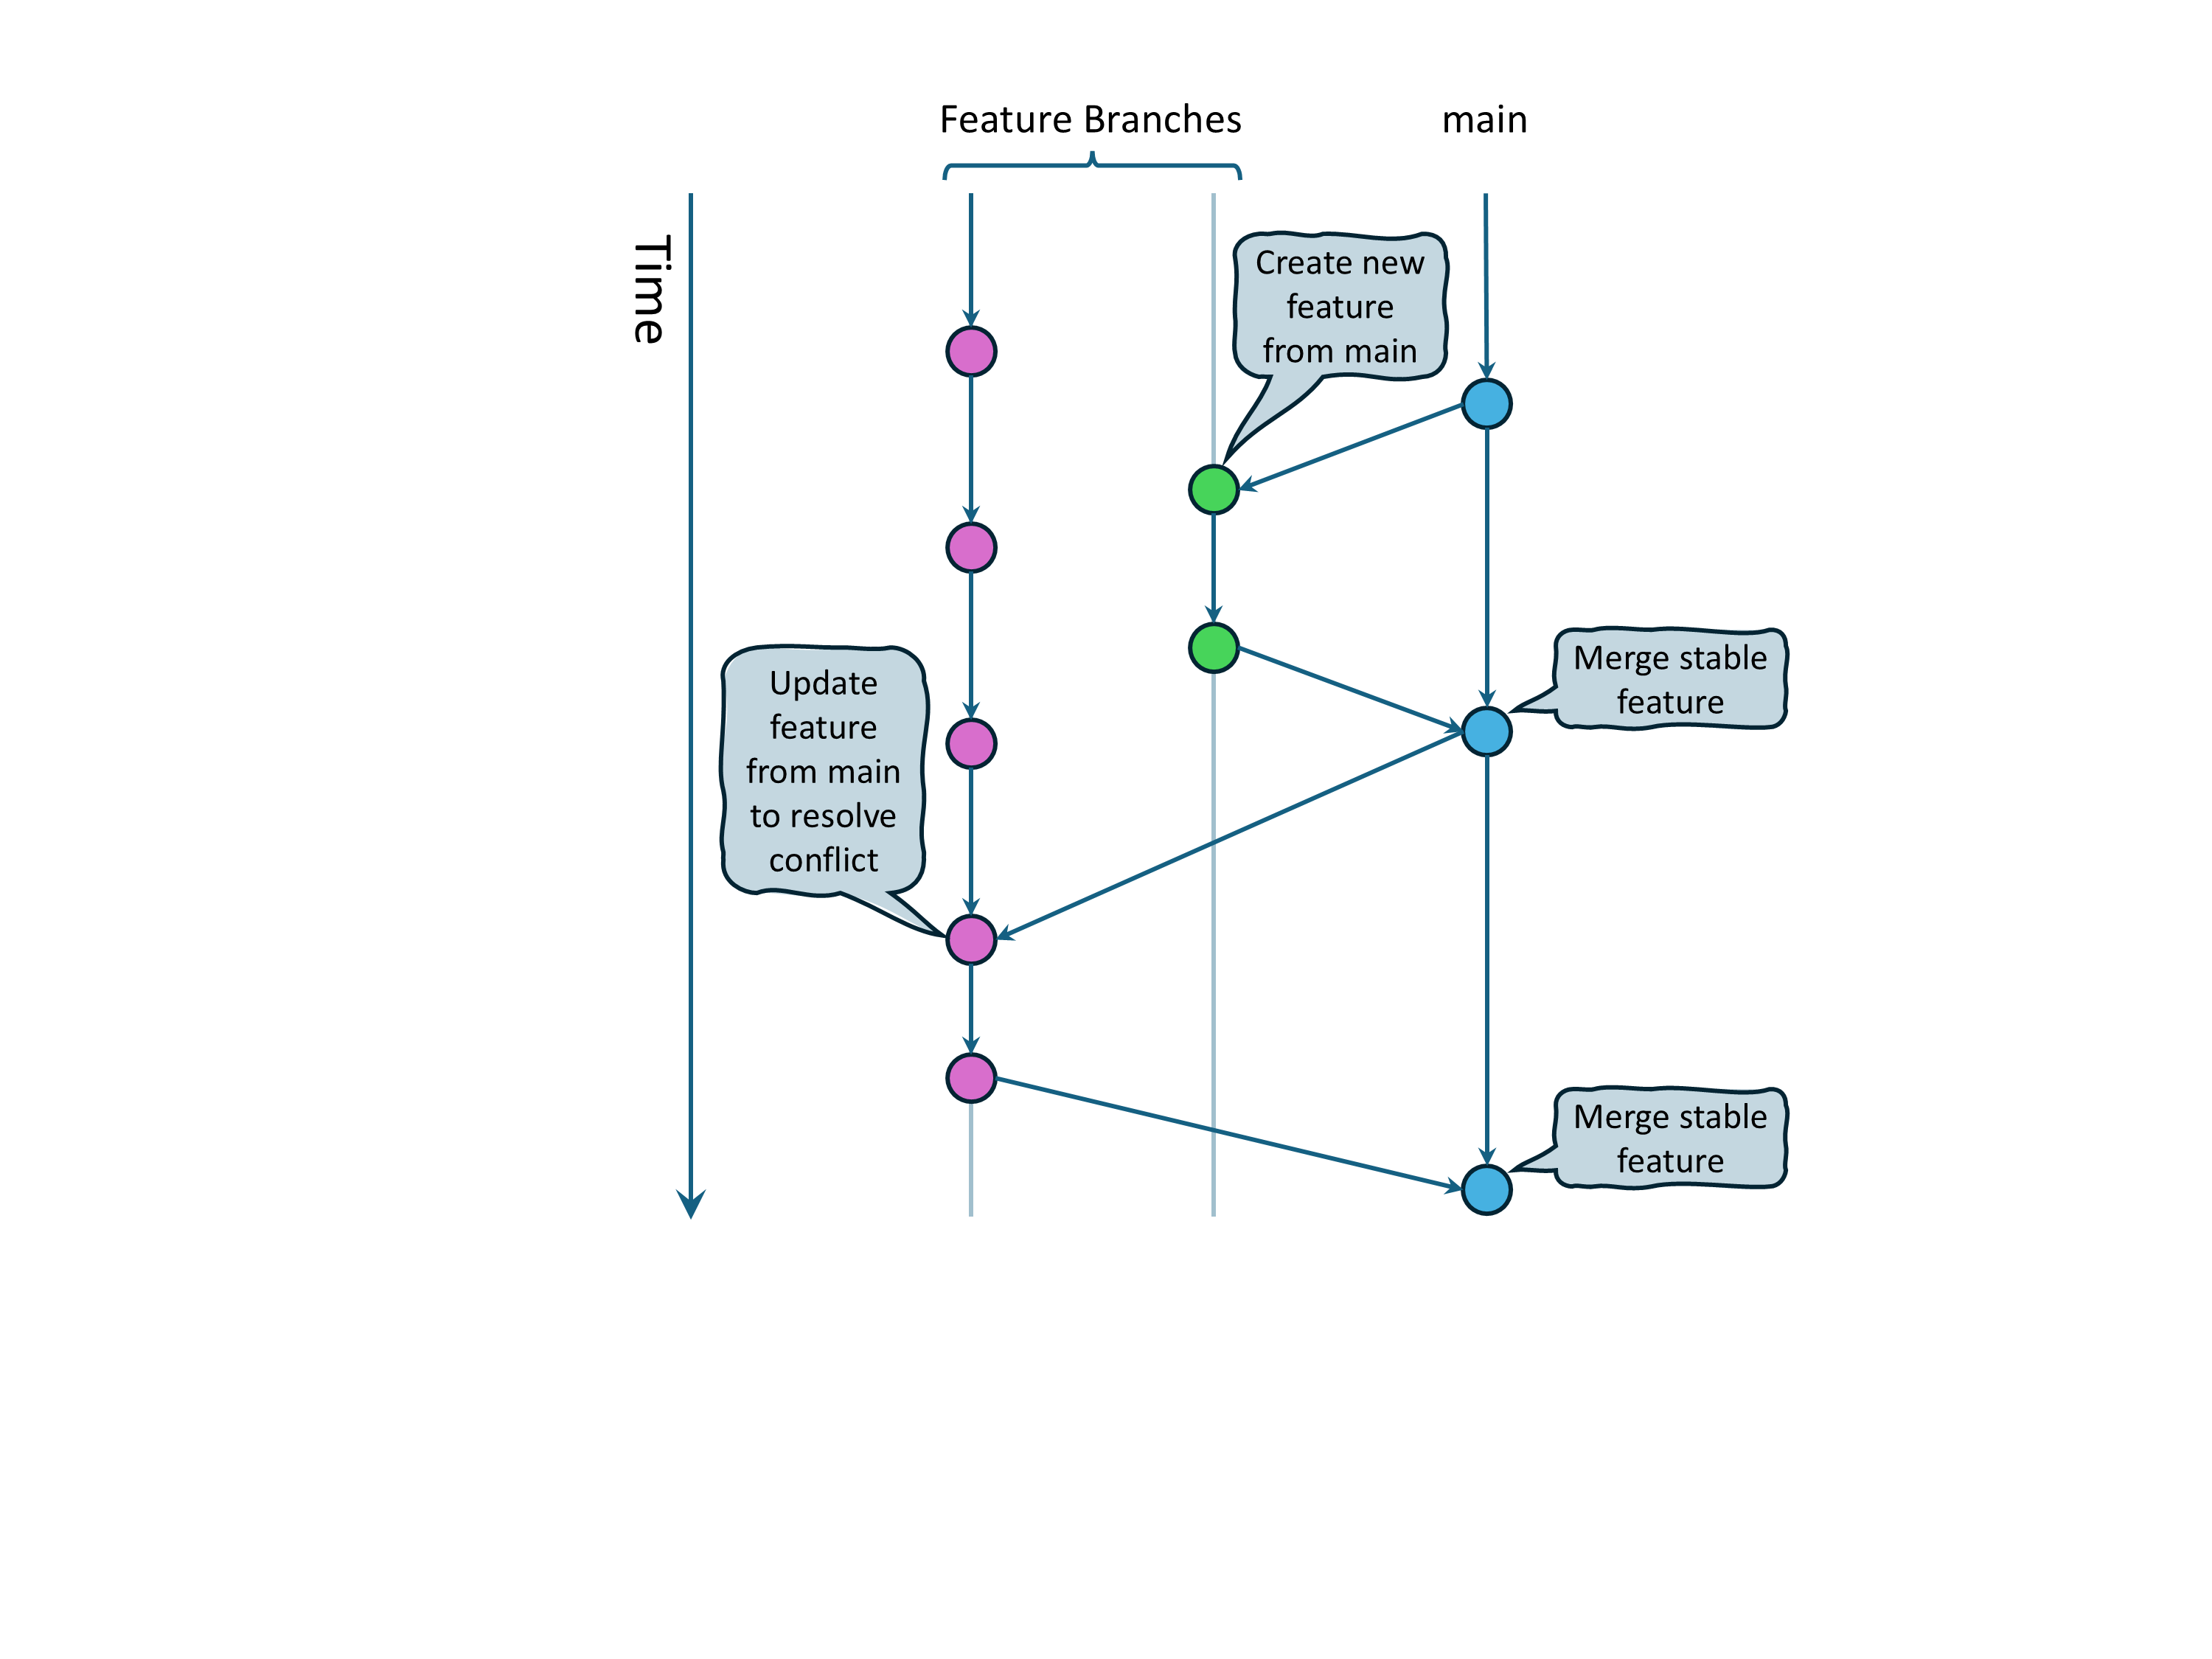
\includegraphics[trim=205 100 125 33,clip,height=\textheight]{diagrams/github-flow}
    \end{columns}
\end{frame}
\note[itemize]{
    \item CSSE3200 Feature Branches are a variant of this.
    \item Supports CI \& CD.
    \item Expects there is a single deployable version\\ (e.g. cloud / web systems).
}

\begin{frame}{GitLab Flow \cite{gitlab-flow}}
    \vspace{1pt}
    \begin{columns}
    \column{0.65\textwidth}
      {\LARGE
        \begin{itemize}
            \item Supports deployment windows
            \begin{itemize}
                \Large\item[$-$] Merge to production
                \vspace{0.5mm}
                \Large\item[$-$] Deploy when allowed
            \end{itemize}
            \vspace{2mm}
            \item Production branch
            \begin{itemize}
                \Large\item[$-$] Plus alpha, beta, \dots
            \end{itemize}
            \vspace{1.5mm}
            \item Still have
            \begin{itemize}
                \Large\item[$-$] Feature branches
                \vspace{0.5mm}
                \Large\item[$-$] Pull requests
            \end{itemize}
        \end{itemize}
      }
    \column{0.35\textwidth}
        \centering
        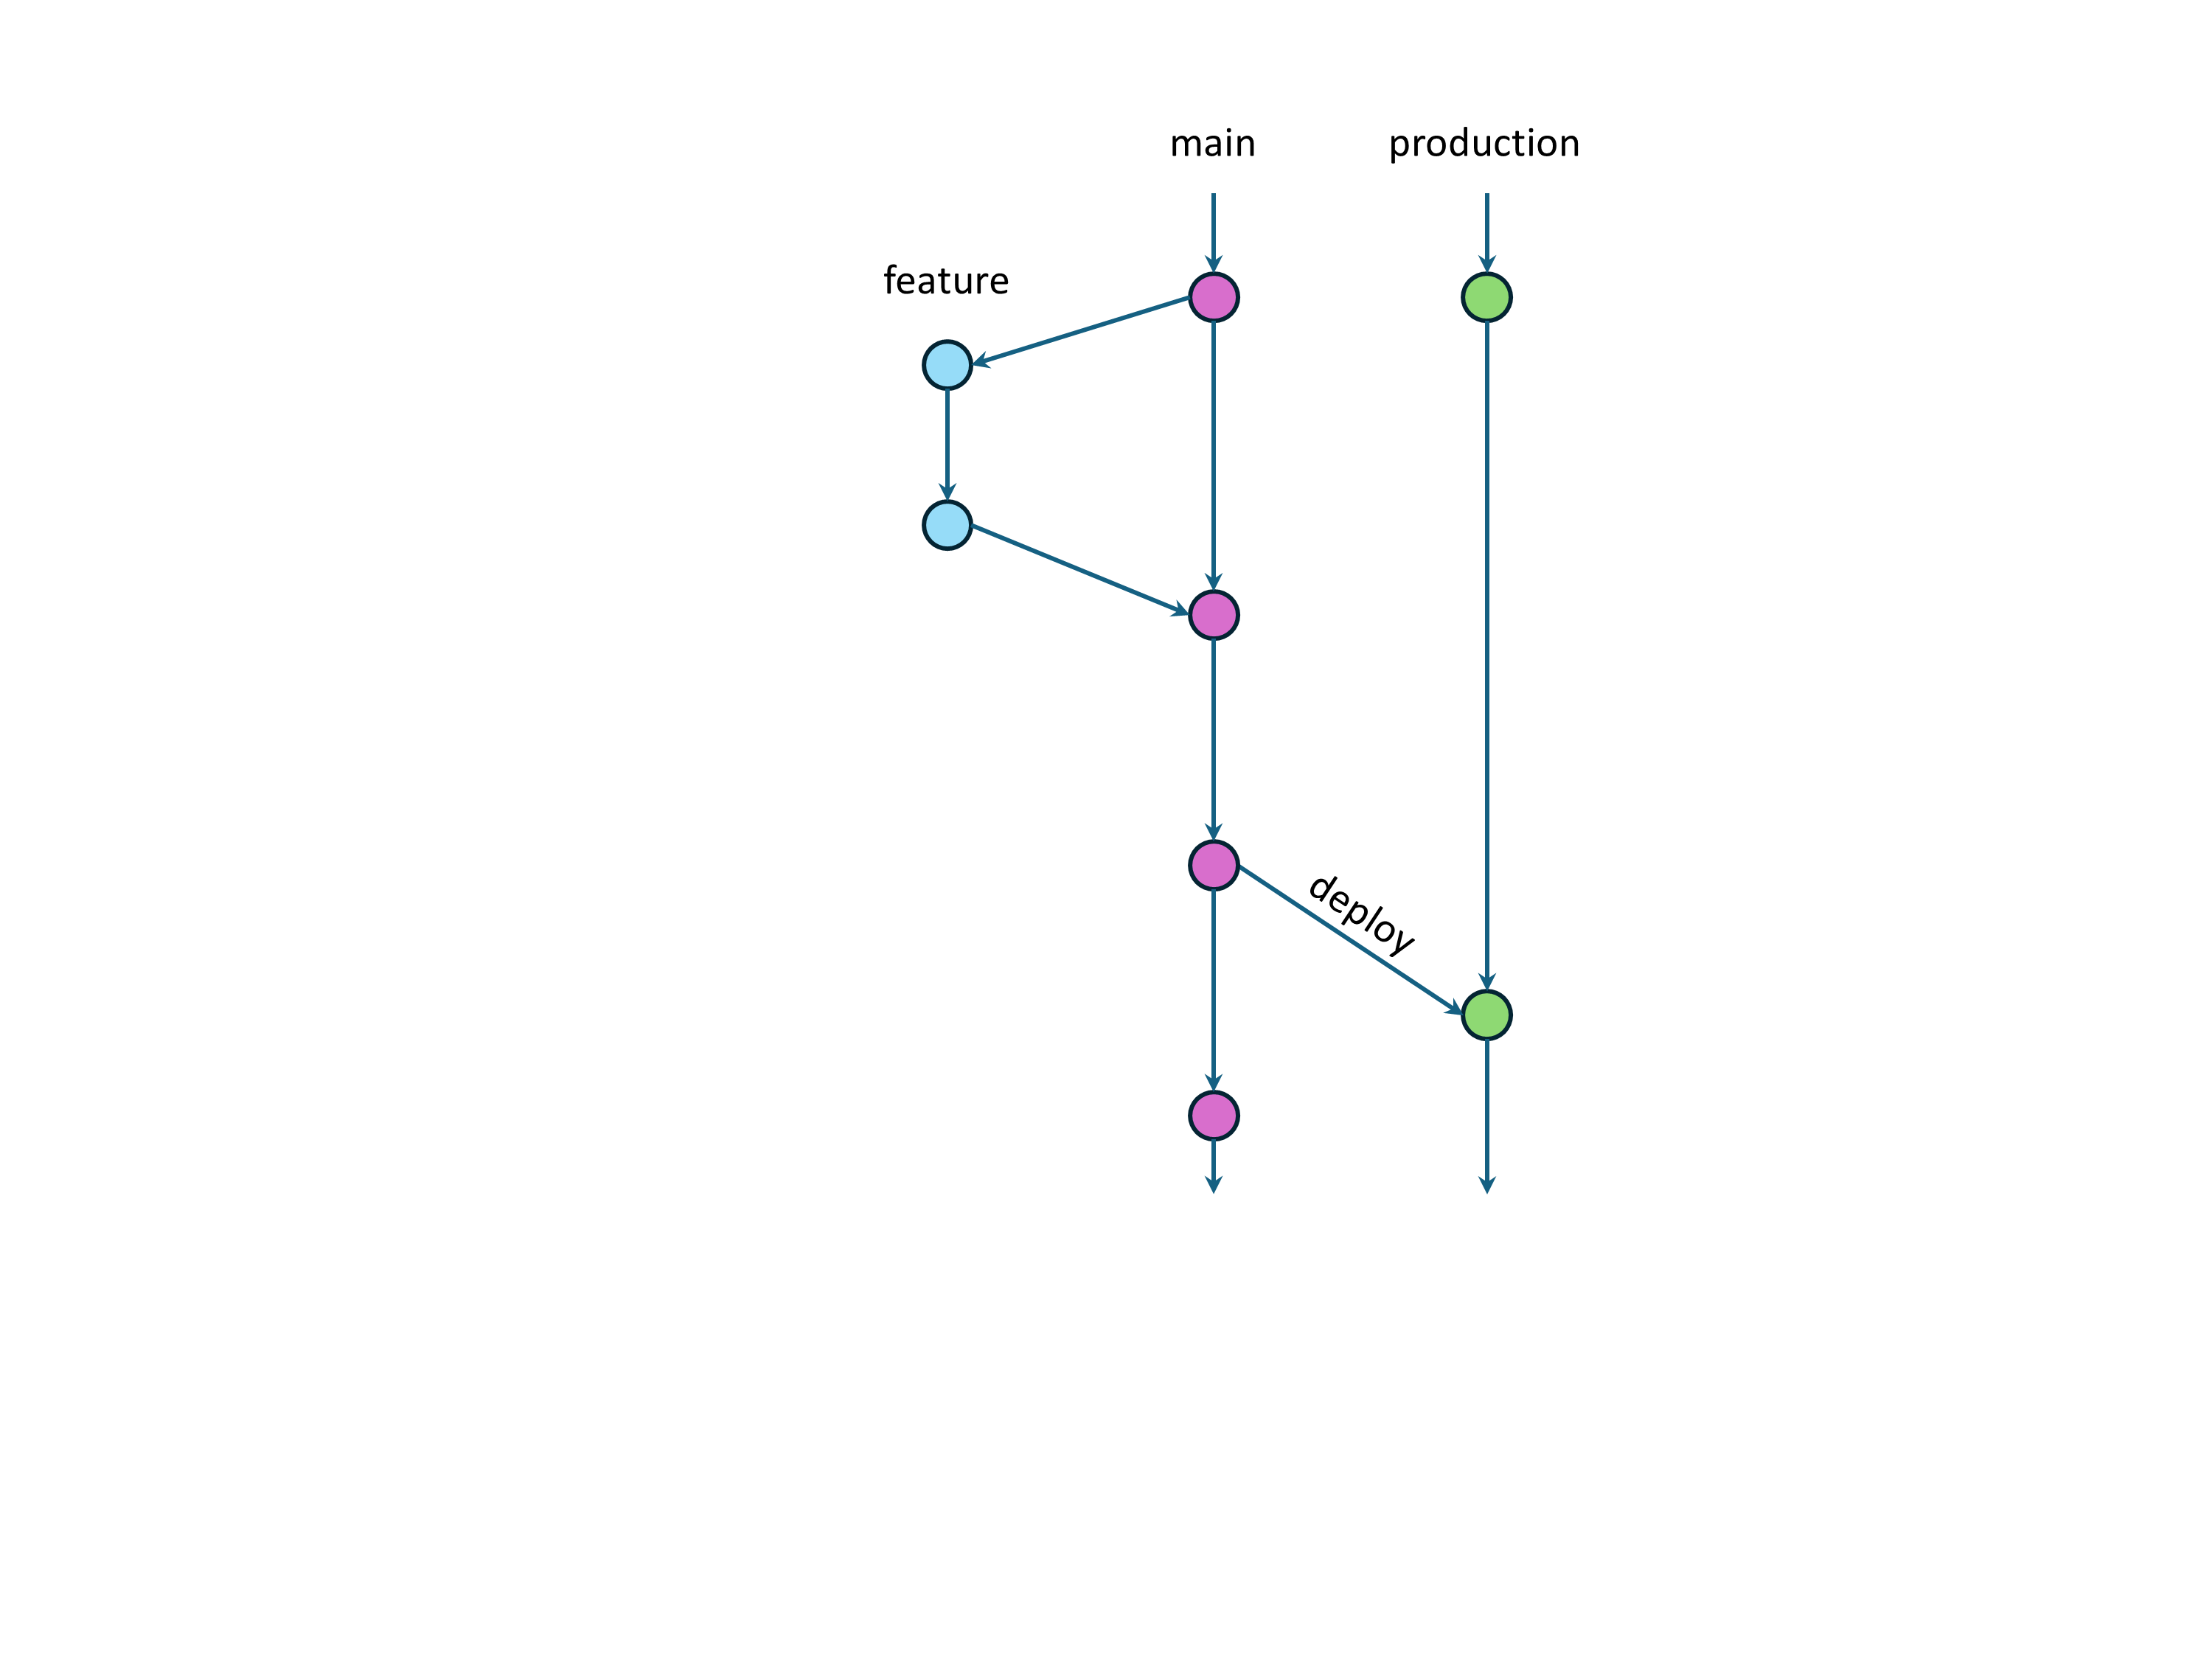
\includegraphics[height=0.9\textheight]{diagrams/gitlab-flow.png}
    \end{columns}
\end{frame}
\note[itemize]{
    \item Deployment windows examples
    \begin{itemize}
        \Large\item App store approval
        \Large\item Server availability
        \Large\item Support availability
    \end{itemize}
}

\begin{frame}{Release Branches \cite{gitlab-flow}}
    \vspace{1pt}
    \begin{columns}
    \column{0.6\textwidth}
      \vspace{-5mm}
      {\LARGE
        \begin{itemize}
            \item {\setstretch{0.95} Supports multiple versions of system\\}
            \item Feature development in main
            \item Released versions are branches
            \vspace{3mm}
            \item Bug fixes in main
            \begin{itemize}
                \Large\item[$-$] Cherry-pick into branches
            \end{itemize}
        \end{itemize}
      }
    \column{0.4\textwidth}
        \centering
        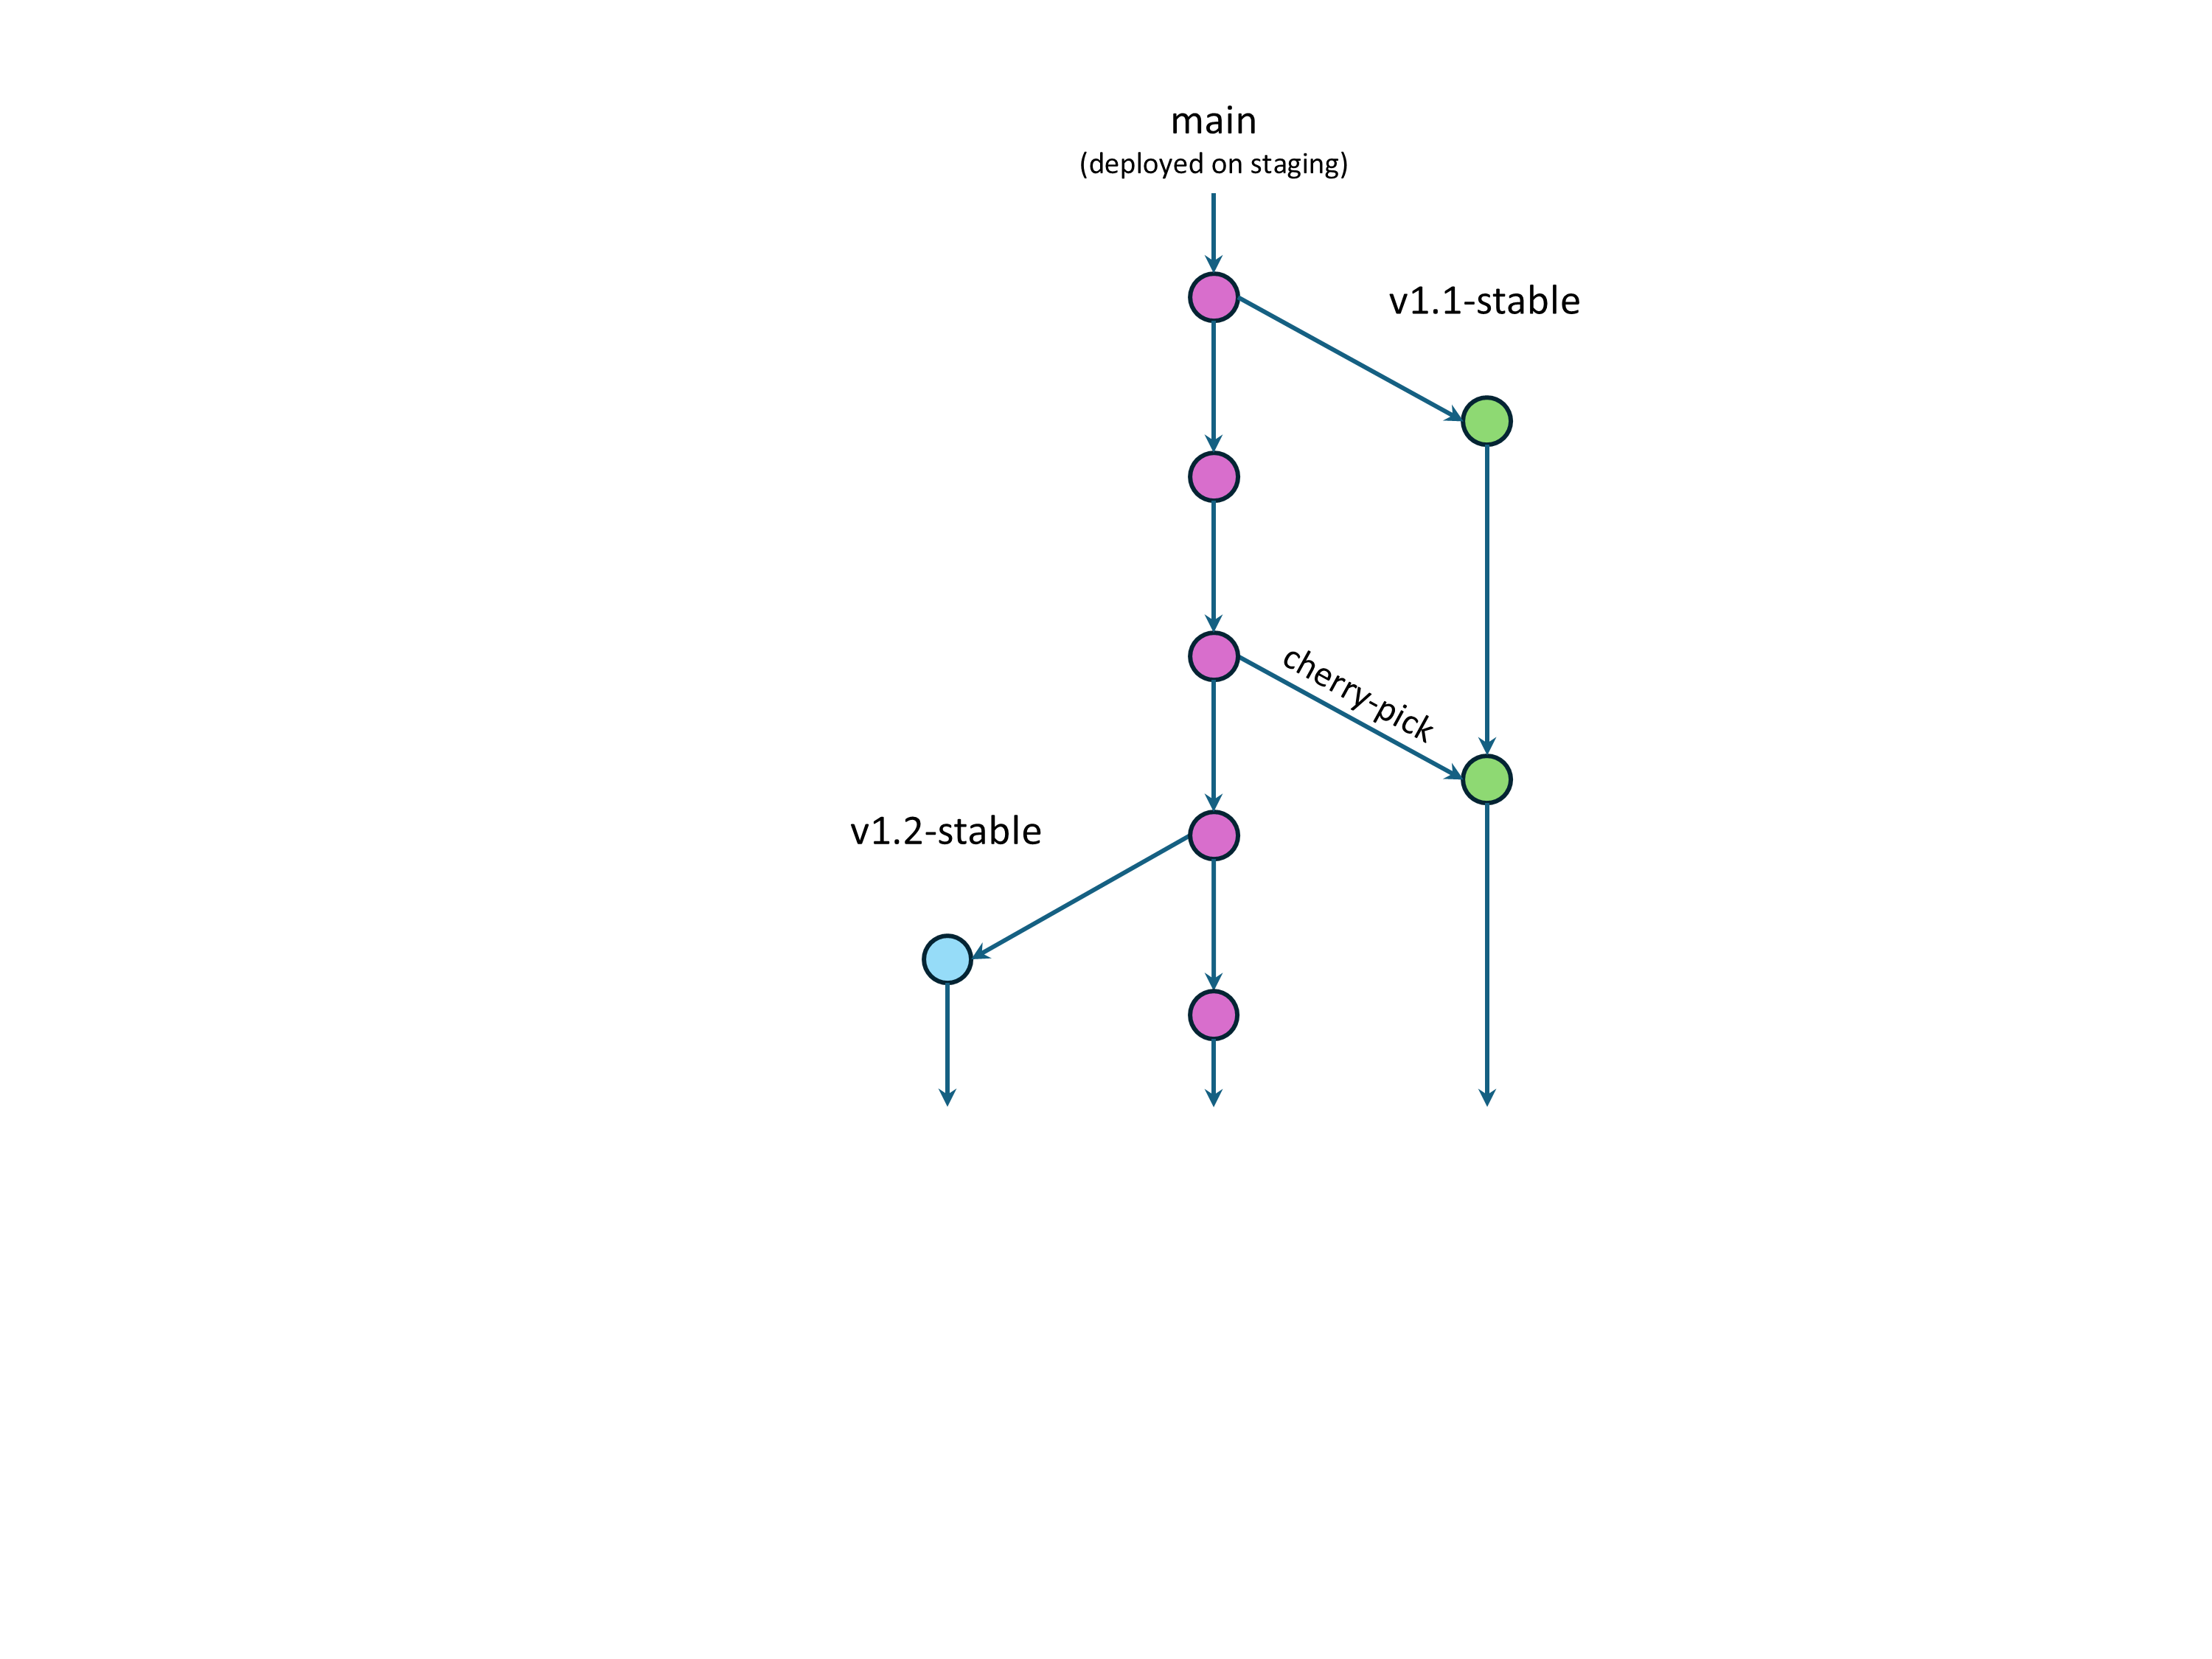
\includegraphics[height=0.9\textheight]{diagrams/release-branches.png}
    \end{columns}
\end{frame}
\note[itemize]{
    \item Cherry-pick: commit is copied from one branch to another, but the branches aren't merged.
}


\definition{Deployment Strategy}{How a software system is made available to clients.}

\begin{frame}{Recreate Deployment \cite{deployment-strategies}}
    \vspace{1pt}
    \centering
    % \animategraphics output only works in Adobe Acrobat.
    % Replace with \includegraphics of the merged image for slides published via GitHub.
%    \animategraphics[trim=10 115 10 100,clip,controls,buttonsize=1em,width=1.05\linewidth]{6}{diagrams/recreate/fnum}{1}{20}
    \includegraphics[height=\textheight]{diagrams/recreate.png}
\end{frame}
\note[itemize]{
    \item Shutdown version 1.
    \item Deploy version 2.
    \item Requires downtime.
}

\begin{frame}{Recreate Deployment}
    \vspace{1pt}
    \begin{columns}[t]
    \column{0.5\textwidth}
      \huge Pros
      {\LARGE
        \begin{itemize}
            \item Easy
            \vspace{2mm}
            \item Renewed state
            \begin{itemize}
                \Large\item[$-$] App reinitialised
	            \vspace{2mm}
                \Large\item[$-$] {\setstretch{0.9} Persistent storage consistent with system version\\}
            \end{itemize}
        \end{itemize}
      }
    \column{0.5\textwidth}
      \huge Cons
      {\LARGE
        \begin{itemize}
            \item Downtime
        \end{itemize}
      }
    \end{columns}
\end{frame}
\note{Renewed state means app is reinitialised and db table structure is consistent with system version.}

\begin{frame}{Rolling Deployment \cite{deployment-strategies}}
    \vspace{1pt}
    \centering
    % \animategraphics output only works in Adobe Acrobat.
    % poster option selects frame to display initially, so shows when not animated. Frame count starts from zero.
    % Replace with \includegraphics of the selected frame for slides published via GitHub, to speed up slide compilation.
    \animategraphics[trim=10 115 10 100,clip,poster=14,controls,buttonsize=1em,width=1.05\linewidth]{6}{diagrams/rolling/fnum}{1}{27}
%    \includegraphics[height=\textheight]{diagrams/rolling/fnum15.png}
\end{frame}
\note[itemize]{
    \item Slowly roll out new version.
    \item Pool of instances of \textbf{V1} behind load balancer.
    \item Deploy an instance of \textbf{V2}.
    \item Add \textbf{V2} instance to pool.
    \item Remove one \textbf{V1} instance from pool.
    \item Continue until \textbf{V2} is fully deployed, replacing \textbf{V1}.
}

\begin{frame}{Rolling Deployment}
    \vspace{1pt}
    \begin{columns}[t]
    \column{0.5\textwidth}
      \huge Pros
      {\LARGE
        \begin{itemize}
            \item Fairly easy
            \vspace{1mm}
            \item {\setstretch{0.95} Slow release of new version\\}
            \begin{itemize}
                \Large\item[$-$] Observe issues
                \vspace{0.7mm}
                \Large\item[$-$] Rollback
            \end{itemize}
            \vspace{1mm}
            \item {\setstretch{0.95} Stateful instances can finish gracefully\\}
            \vspace{1mm}
            \begin{itemize}
                \Large\item {\setstretch{0.9} Instance is killed when inactive\\}
            \end{itemize}
        \end{itemize}
      }
    \column{0.5\textwidth}
      \huge Cons
      {\LARGE
        \begin{itemize}
            \item Time
            \item Support multiple APIs
            \item {\setstretch{0.95} Support different versions of persistent data structure\\}
            \item {\setstretch{0.95} No control over traffic to different versions\\}
        \end{itemize}
      }
    \end{columns}
\end{frame}

\begin{frame}{Blue-Green Deployment \cite{deployment-strategies}}
    \vspace{1pt}
    \centering
    % \animategraphics output only works in Adobe Acrobat.
    % poster option selects frame to display initially, so shows when not animated. Frame count starts from zero.
    % Replace with \includegraphics of the selected frame for slides published via GitHub, to speed up slide compilation.
    \animategraphics[trim=10 115 10 100,clip,poster=9,controls,buttonsize=1em,width=1.05\linewidth]{4}{diagrams/blue-green/fnum}{1}{14}
%    \includegraphics[height=\textheight]{diagrams/blue-green/fnum10.png}
\end{frame}
\note[itemize]{
    \item \textbf{V2} deployed alongside \textbf{V1}, including same number of instances.
    \item \textbf{V2} tested in production environment.
    \item Load balancer switched to use \textbf{V2} instances
    \item Shutdown \textbf{V1} instances.
}

\begin{frame}{Blue-Green Deployment}
    \vspace{1pt}
    \begin{columns}[t]
    \column{0.5\textwidth}
      \huge Pros
      {\LARGE
        \begin{itemize}
            \item {\setstretch{0.95} Instant release of new version\\}
            \item Fast rollback if necessary
            \vspace{1mm}
            \item {\setstretch{0.95} Only one version `live' at any time\\}
            \begin{itemize}
                \Large\item[$-$] No versioning conflicts
            \end{itemize}
        \end{itemize}
      }
    \column{0.5\textwidth}
      \huge Cons
      {\LARGE
        \vspace{3mm}
        \begin{itemize}
            \item Expensive
            \begin{itemize}
                \Large\item[$-$] Double the infrastructure
            \end{itemize}
            \vspace{1mm}
            \item {\setstretch{0.95} Stateful instance version switch difficult\\}
            \begin{itemize}
                \Large\item[$-$] Can't kill instance in middle of a transaction
            \end{itemize}
        \end{itemize}
      }
    \end{columns}
\end{frame}

\begin{frame}{Canary Deployment \cite{deployment-strategies}}
    \vspace{1pt}
    \centering
    % \animategraphics output only works in Adobe Acrobat.
    % poster option selects frame to display initially, so shows when not animated. Frame count starts from zero.
    % Replace with \includegraphics of the selected frame for slides published via GitHub, to speed up slide compilation.
    \animategraphics[trim=10 115 10 100,clip,poster=13,controls,buttonsize=1em,width=1.05\linewidth]{4}{diagrams/canary/fnum}{1}{15}
%    \includegraphics[height=\textheight]{diagrams/canary/fnum14.png}
\end{frame}
\note[itemize]{
    \item Gradually shift traffic from \textbf{V1} to \textbf{V2}.
    \item Traffic usually split by percent (e.g. 90/10, 80/20, ...).
    \item Allows a trial deployment to see what happens.
}

\begin{frame}{Canary Deployment}
    \vspace{1pt}
    \begin{columns}[t]
    \column{0.5\textwidth}
      \huge Pros
      {\LARGE
        \begin{itemize}
            \item {\setstretch{0.95} New version released to subset of users\\}
            \item {\setstretch{0.95} Can monitor perform- ance and error rates\\}
            \item Easy and fast rollback
        \end{itemize}
      }
    \column{0.5\textwidth}
      \huge Cons
      {\LARGE
        \begin{itemize}
            \item Slow
            \item Implies poor testing
        \end{itemize}
      }
    \end{columns}
\end{frame}
\note{Canary is commonly used to see if something works or will fail in production.}

\begin{frame}{A/B Deployment \cite{deployment-strategies}}
    \vspace{1pt}
    \centering
    % \animategraphics output only works in Adobe Acrobat.
    % poster option selects frame to display initially, so shows when not animated. Frame count starts from zero.
    % Replace with \includegraphics of the selected frame for slides published via GitHub, to speed up slide compilation.
    \animategraphics[trim=10 115 10 100,clip,poster=last,controls,buttonsize=1em,width=1.05\linewidth]{6}{diagrams/a-b/fnum}{1}{19}
%    \includegraphics[height=\textheight]{diagrams/a-b/fnum19.png}
\end{frame}
\note[itemize]{
    \item Actually it's A/B Testing.
    \item Both versions are deployed and usage evaluated, usually via analytics.
    \item Long Term: Deploy version that has best usage result.
}

\begin{frame}{A/B Deployment}
    \vspace{1pt}
    \begin{columns}[t]
    \column{0.5\textwidth}
      \huge Pros
      {\LARGE
        \begin{itemize}
            \item {\setstretch{0.95} Multiple versions run in parallel\\}
            \vspace{1mm}
            \item {\setstretch{0.95} Full control over traffic distribution\\}
        \end{itemize}
      }
    \column{0.5\textwidth}
      \huge Cons
      {\LARGE
        \begin{itemize}
            \item {\setstretch{0.95} Needs intelligent load balancer\\}
            \vspace{1mm}
            \item {\setstretch{0.95} Debugging a version is difficult\\}
            \begin{itemize}
                \Large\item[$-$] Need good logs \& tools
            \end{itemize}
        \end{itemize}
      }
    \end{columns}
\end{frame}
\note{A/B testing \& deployment requires sophisticated infrastructure and analytics to do well.}

\begin{frame}{Shadow Deployment \cite{deployment-strategies}}
    \vspace{1pt}
    \centering
    % \animategraphics output only works in Adobe Acrobat.
    % poster option selects frame to display initially, so shows when not animated. Frame count starts from zero.
    % Replace with \includegraphics of the selected frame for slides published via GitHub, to speed up slide compilation.
    \animategraphics[trim=10 115 10 100,clip,poster=13,controls,buttonsize=1em,width=1.05\linewidth]{5}{diagrams/shadow/fnum}{1}{15}
%    \includegraphics[height=\textheight]{diagrams/shadow/fnum14.png}
\end{frame}
\note[itemize]{
    \item Complex to setup.
    \item \textbf{V2} deployed alongside \textbf{V1}.
    \item All traffic is sent to \textbf{V1} \& \textbf{V2}.
    \item Tests \textbf{V2} ability to handle production load.
    \item Doesn't impact on production traffic or user experience.
    \item \textbf{V2} rolled out when it demonstrates it is stable.
    \item Need to manage interactions with external services\\ (e.g. payment gateway).
    \item When customer checks out their shopping cart,
          you don't want to send two payment requests from \textbf{V1} \& \textbf{V2}.
    \item Mock external services.
    \item Persistent data from \textbf{V1} (production data) needs to be copied to \textbf{V2}
          when it's deployed as production, with any data migration.
}

\begin{frame}{Shadow Deployment}
    \vspace{1pt}
    \begin{columns}[t]
    \column{0.5\textwidth}
      \huge Pros
      {\LARGE
        \begin{itemize}
            \item {\setstretch{0.95} Performance testing with production traffic\\}
            \item No impact on users
        \end{itemize}
      }
    \column{0.5\textwidth}
      \huge Cons
      {\LARGE
        \vspace{3mm}
        \begin{itemize}
            \item Expensive
            \begin{itemize}
                \Large\item[$-$] Double the infrastructure
            \end{itemize}
            \vspace{2mm}
            \item Complex to setup
            \begin{itemize}
                \Large\item[$-$] Need mocks for external services
            \end{itemize}
        \end{itemize}
      }
    \end{columns}
\end{frame}
\note{Performance testing may give false confidence.\\ ~~~-- It's not user testing.}

\begin{frame}{Deployment Strategy Options}
  \vspace{1pt}
  {\huge
    \begin{itemize}
        \item Staging or beta testing
        \begin{itemize}
            \LARGE\item[$-$] Recreate or Rolling
        \end{itemize}
        \vspace{1mm}
        \item Production (Live)
        \begin{itemize}
            \LARGE\item[$-$] Rolling or Blue/Green
        \end{itemize}
        \vspace{1mm}
        \item Uncertain of system stability
        \begin{itemize}
            \LARGE\item[$-$] Canary
        \end{itemize}
        \vspace{1mm}
        \item Evaluation
        \begin{itemize}
            \LARGE\item[$-$] A/B or Shadow
        \end{itemize}
    \end{itemize}
  }
\end{frame}
\note{There isn't any one perfect deployment strategy.}

\begin{frame}{Deployment Considerations \cite{deployment-strategies}}
    \centering
    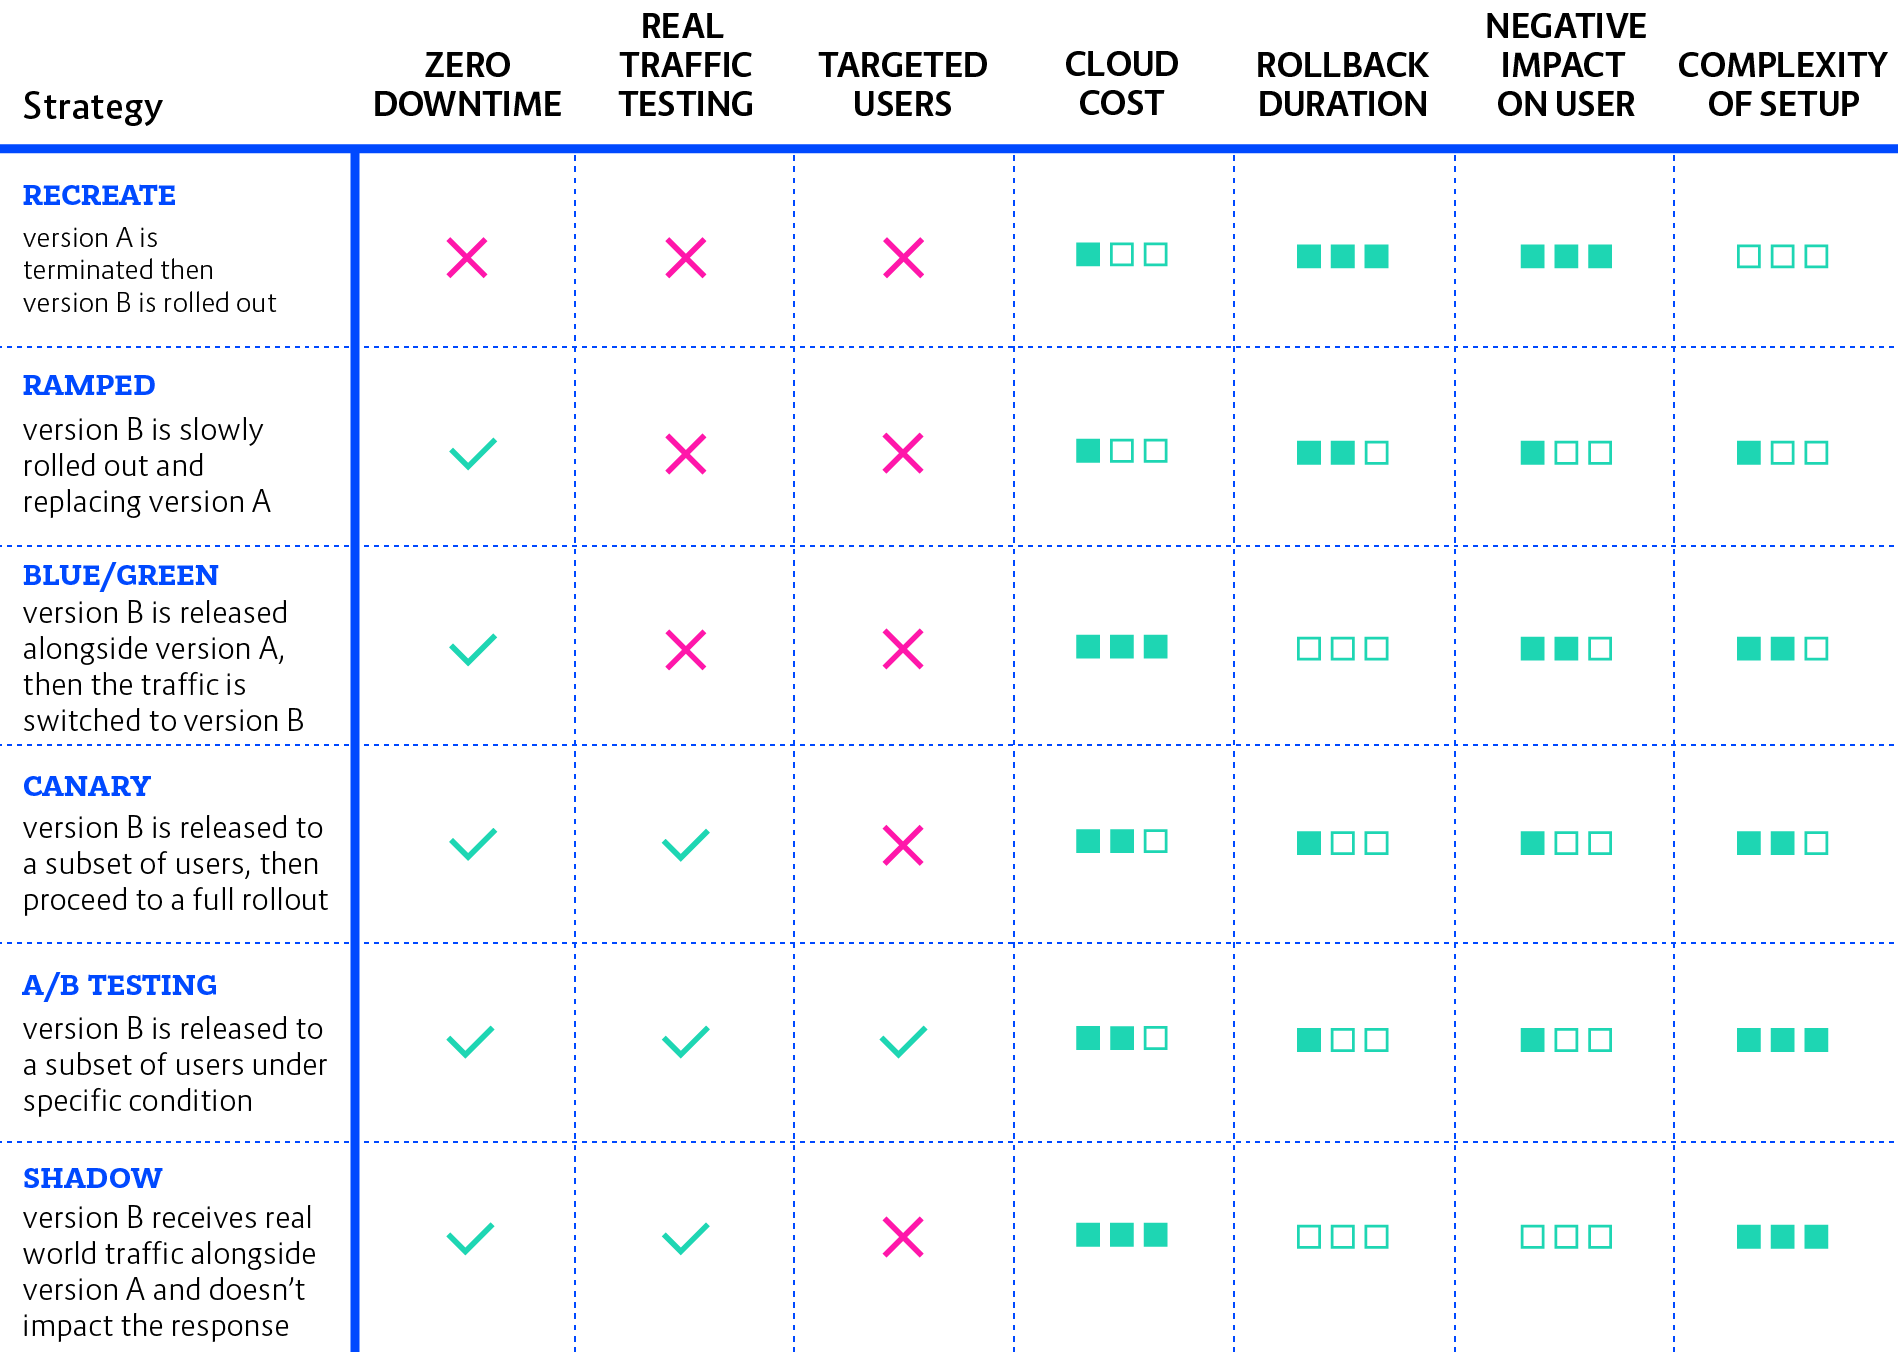
\includegraphics[height=0.93\textheight]{diagrams/deployment_strategies.png}
\end{frame}

% Manually created table of deployment_strategies.png content.
%\begin{frame}{Deployment Considerations}
%\vspace{-10mm}
%\begin{table}
%\begin{adjustwidth}{-12mm}{-12mm}
%\centering
%% Figure out how to fix first row's text having double-line spacing after line break.
%\def\arraystretch{1.5}
%\begin{tabular}{lccccccc}
%\rowcolor[rgb]{0.835,1,0.835} \multicolumn{1}{c}{Strategy} & \begin{tabular}[c]{@{}>{\cellcolor[rgb]{0.835,1,0.835}}c@{}}Zero\\Downtime\end{tabular} & \begin{tabular}[c]{@{}>{\cellcolor[rgb]{0.835,1,0.835}}c@{}}Real\\Traffic\end{tabular} & \begin{tabular}[c]{@{}>{\cellcolor[rgb]{0.835,1,0.835}}c@{}}Targeted\\Users\end{tabular} & Cost   & \begin{tabular}[c]{@{}>{\cellcolor[rgb]{0.835,1,0.835}}c@{}}Rollback\\Duration\end{tabular} & \begin{tabular}[c]{@{}>{\cellcolor[rgb]{0.835,1,0.835}}c@{}}Impact\\on Users\end{tabular} & \begin{tabular}[c]{@{}>{\cellcolor[rgb]{0.835,1,0.835}}c@{}}Setup\\Complexity\end{tabular}  \\
%\rowcolor[rgb]{0.941,1,1} Recreate                         & N                                                                                       & N                                                                                      & N                                                                                         & \$     & Long                                                                                        & High                                                                                      & Negligible                                                                                  \\
%\rowcolor[rgb]{1,0.937,1} Rolling                          & Y                                                                                       & N                                                                                      & N                                                                                         & \$     & Long                                                                                        & Low                                                                                       & Low                                                                                         \\
%\rowcolor[rgb]{0.941,1,1} Blue/Green                       & Y                                                                                       & N                                                                                      & N                                                                                         & \$\$\$ & Negligible                                                                                  & Medium                                                                                    & Medium                                                                                      \\
%\rowcolor[rgb]{1,0.937,1} Canary                           & Y                                                                                       & Y                                                                                      & N                                                                                         & \$     & Short                                                                                       & Low                                                                                       & Medium                                                                                      \\
%\rowcolor[rgb]{0.941,1,1} A/B Testing                      & Y                                                                                       & Y                                                                                      & Y                                                                                         & \$\$   & Short                                                                                       & Low                                                                                       & High                                                                                        \\
%\rowcolor[rgb]{1,0.937,1} Shadow                           & Y                                                                                       & Y                                                                                      & N                                                                                         & \$\$\$ & Negligible                                                                                  & Negligible                                                                                & High                                                                                       
%\end{tabular}
%\end{adjustwidth}
%\end{table}
%\end{frame}

\references{deployment}

\end{document}